\documentclass[a4paper,BCOR7mm,12pt,pointlessnumbers,bibtotoc]{scrartcl}
% Define German as thesis language
%\usepackage{german}

\usepackage{latexsym,alltt,
            textcomp, float}

% Codierung
\usepackage[latin1]{inputenc}

% zusaetzliche Symbole
\usepackage{textcomp, latexsym}

% Grafiken
\usepackage{graphicx, psfrag}

% "H"-Option für Gleitumgebungen
\usepackage{float}

% Gleitumgebungen nach Referenz platzieren
\usepackage{flafter}

% lange Tabellen
\usepackage{longtable}

%Mathematik
\usepackage{amsmath}
\usepackage{amsfonts}
\usepackage{amssymb}

% pdftex
\usepackage{hyperref}

% neue deutsche Rechtschreibung
%\usepackage{ngerman}

% zusätzliche Spaltendefinitionen für Tabellen
\usepackage{array}

% Darstellung mehrerer Bilder als ein Objekt
\usepackage{subfigure}

% Drehen von Grafiken (turn,rotate)
\usepackage{rotating}
 
% Weitere Symbole
%\usepackage{psnfss}
\usepackage{pifont}

%Farben
\usepackage{color}

% Absatzabstand etwas groesser
\addtolength{\parskip}{1.1ex}

% Blocksatz erzwingen
\sloppy

% Abstand zweier Listenelemente kleiner
\setlength{\itemsep}{0ex plus0.2ex}

% "Rahmenabstand" für gerahmte Gleichungen
\setlength{\fboxsep}{10pt}

\begin{document}
%\maketitle
\begin{center}
\Large Direct Digital Synthesizer IP Core\\[0.4cm]
\large Martin Kumm \\[0.5cm]
\large \today \\[0.5cm]
%\Large 19.12.2007 \\[1.0cm]
\end{center}

%\tableofcontents
%\newpage

The DDS IP core (\verb|dds_synthesizer|) is a implementation of a direct digital frequency synthesizer (DDS) (also called number controlled oscillator, NCO) which produces a sinewave at the output with a specified frequency and phase (adjustable at runtime). The resolution of the frequency tuning word (FTW), the phase and the amplitude are defined seperately. While the FTW resolution can be set by the generic \verb|ftw_width|, phase and amplitude resolution are defined as constants \verb|phase_width| and \verb|ampl_width| in the seperate package \verb|sine_lut_pkg|. This is generated by a matlab script (\verb|matlab/sine_lut_gen.m|), the m-files are described in their headers. The most relevant LUTs (in the range 8...16Bit) have been generated and are located in the ``\verb|VHDL/sine_lut|'' folder. The nomenclature of the files is \verb|sine_<phase_width>_x_<amplitude_width>_pkg.vhd|. By adding one of these files to the project, the resolution of phase and amplitude is automatically defined.

Figure 1 shows a block diagram of the implemented DDS synthesizer. The signals \verb|clk| and \verb|reset| are not shown here. The resolution parameters have been renamed (\verb|ftw_width|=N, \verb|phase_width|=M and \verb|amplitude_width|=P). Only the first period of the sinewave is stored in the LUT, the two most significant bits of the phase word are used either to shift the input value or to invert the output amplitude, depending on the quadrant of the sinewave. The LUT is clocked, so the total delay from input to output is 3 clock cycles. 
\begin{figure}[H]
  \centering
    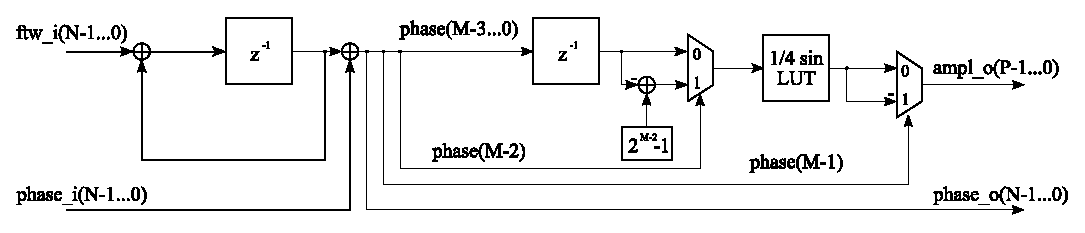
\includegraphics[width=14cm]{images/dds_implementation}
  \caption{Block diagram of the DDS implementation}
  \label{fig:dds_implementation}
\end{figure}

The output frequency will be determined by the FTW (\verb|ftw_i|)
\begin{equation}
  f_{DDS}=\frac{FTW}{2^M} f_s \ \ .
  \label{equ:ftw}
\end{equation}
The initial phase (when using more than one synthesizer) can be set by setting the PTW (\verb|phase_i|) to
\begin{equation}
  \varphi_{DDS}=\frac{PTW}{2^N} 2 \pi \ \ .
  \label{equ:ptw}
\end{equation}

A Testbench is realized in \verb|dds_synthesizer_tb.vhd|, the corresponding Modelsim project can be found in the \verb|/sim| folder. The ports of the entity are described in Table~\ref{tab:ports}.

\begin{table}[H]
  \centering
    \begin{tabular}{l|c|c|l}
      \hline
      \hline
        Name & Direction & Wordsize & Description \\
        \hline
        \verb|clk_i|   & \verb|in|  & 1                  & clock \\
        \verb|rst_i|   & \verb|in|  & 1                  & reset  \\
        \verb|ftw_i|   & \verb|in|  & \verb|ftw_width|   & Frequency Tuning Word, see Formula (\ref{equ:ftw})  \\
        \verb|phase_i| & \verb|in|  & \verb|phase_width| & Phase Tuning Word, see Formula (\ref{equ:ptw})  \\
        \verb|phase_o| & \verb|out| & \verb|phase_width| & Instantaneous Phase Output  \\
        \verb|ampl_o|  & \verb|out| & \verb|ampl_width | & Amplitude Output  \\
      \hline
      \hline
    \end{tabular}
  \caption{Entity port description}
  \label{tab:ports}
\end{table}

%\bibliographystyle{alpha}
%\bibliography{dsp_4_sdr}

\end{document}


 
